\noindent
{\Large \textbf{\section{Анализ клеточного автомата}}} \par


\noindent{\Large \textbf{\subsection{Паттерны}}} \par

\noindent{\large \textbf{\subsubsection{Тривиальные начальные условия}}} \par

Для начала рассмотрим два тривиальных начальных условия, когда все клетки или одновременно живы, или мертвы.

Пустое поле неподвижно, так как $f(0,0,0,0,0)=0$, а полностью заполненное поле за один шаг становится пустым, так как $f(1,1,1,1,1)=0$.

При нетривиальных начальных условиях можно выделить два вида поведения: шахматные доски, которые на каждой итерации инвертируют клетки, и диагональные волны, которые дрейфуют по полю. Рассмотрим их отдельно.

{\large \textbf{\subsubsection{Шахматные доски}}} \par

Существуют две шахматные доски: с живой и с мертвой клеткой в левом верхнем углу. В любой из них все четыре соседа каждой клетки имеют цвет, противоположный цвету самой клетки, поэтому используются только две строки таблицы истинности:
\begin{itemize}[itemsep=-3pt]
 \item живая клетка с мертвыми соседями, $f(0,0,1,0,0)=0$ ($i=4$): клетка умирает
 \item мертвая клетка с живыми соседями, $f(1,1,0,1,1)=1$ ($i=27$): клетка оживает
\end{itemize}
Следовательно, на каждом шаге все клетки меняют цвет, $x_{t+1}=1-x_t$: одна доска заменяется другой, а через два шага возвращается в исходное состояние, то есть пара шахматных досок образует цикл периода $2$ шага (рис.\ref{fig:checker}).

Однако цвета чередуются в шахматном порядке только при чётной ширине поля из-за тороидальных граничных условий.
При нечетной ширине поля, после нескольких итераций поле прийдет к паттерну дрейфующих волн, описанному ниже.

\begin{figure}[H]
 \centering
 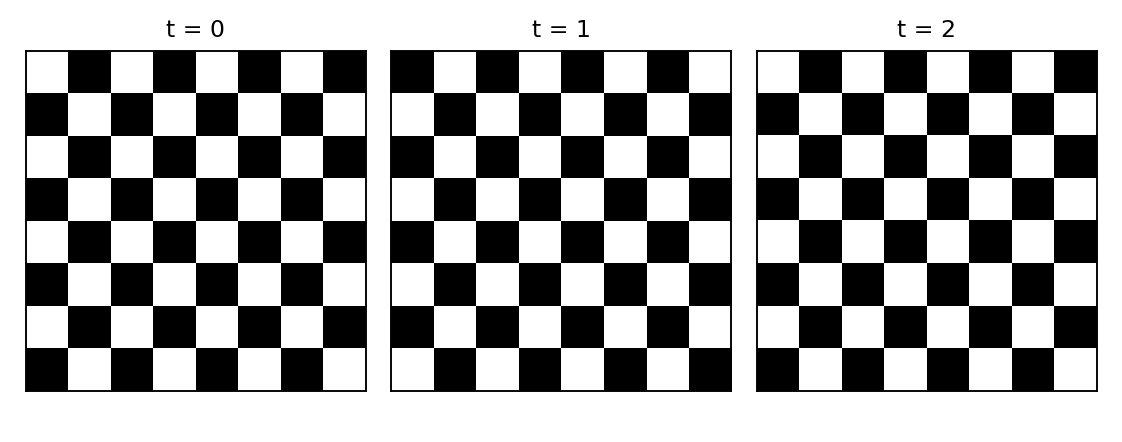
\includegraphics[width=0.55\textwidth]{pic/checkerboard.png}
 \caption{Шахматное поле $8\times 8$: цикл периода 2}
 \label{fig:checker}
\end{figure}

{\large \textbf{\subsubsection{Диагональные волны (дрейф вправо)}}} \par

В отличие от шахматных досок, здесь закрашенные клетки не стоят на месте, а смещаются вправо, закрашивая соседа по диагонали. Наиболее чистый пример даёт одиночная живая клетка (рис.\ref{fig:drift}).

Таким образом, на каждом шаге живая клетка исчезает, но передаёт жизнь соседу справа и соседу снизу. Эти две новые клетки лежат на одной диагонали, поэтому из одной клетки возникает диагональный отрезок. 

Волна на торе ширины $n$ замыкается при $t=n-1$, диагональ при этом состоит из $n$ клеток.

\begin{figure}[H]
 \centering
 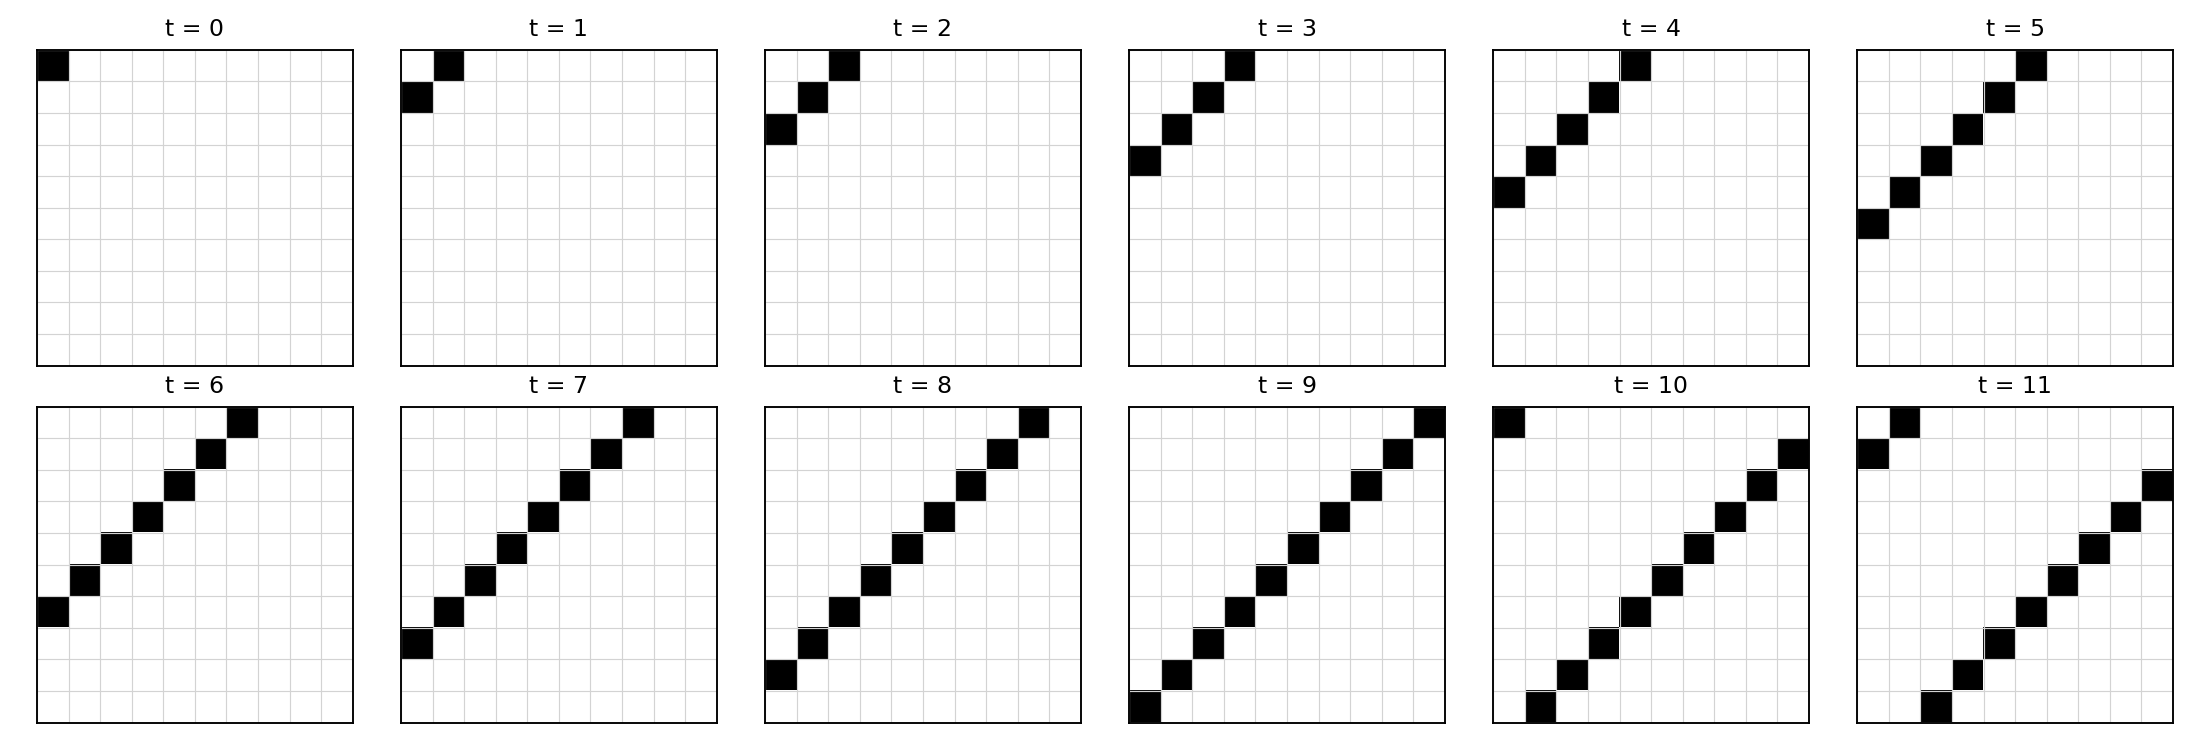
\includegraphics[width=\textwidth]{pic/drift.png}
 \caption{Диагональная волна на торе $10\times 10$}
 \label{fig:drift}
\end{figure}


% \noindent{\Large \textbf{\subsection{Плотность}}} \par

% Доля живых клеток быстро выходит на уровень около $0{,}5$ и далее лишь слабо колеблется (рис.\ref{fig:density}). При случайном старте с плотностью $1/2$ в аттракторе она лежит в пределах $0{,}46$-$0{,}54$. Если начальная плотность сильно отличается от $1/2$, система все равно «стягивается» к середине, но не полностью: плотность при $t=200$ составляет около $0{,}39$ при старте $0{,}05$ и около $0{,}34$ при старте $0{,}95$ (рис.\ref{fig:density_init}).

% \begin{figure}[H]
%  \centering
%  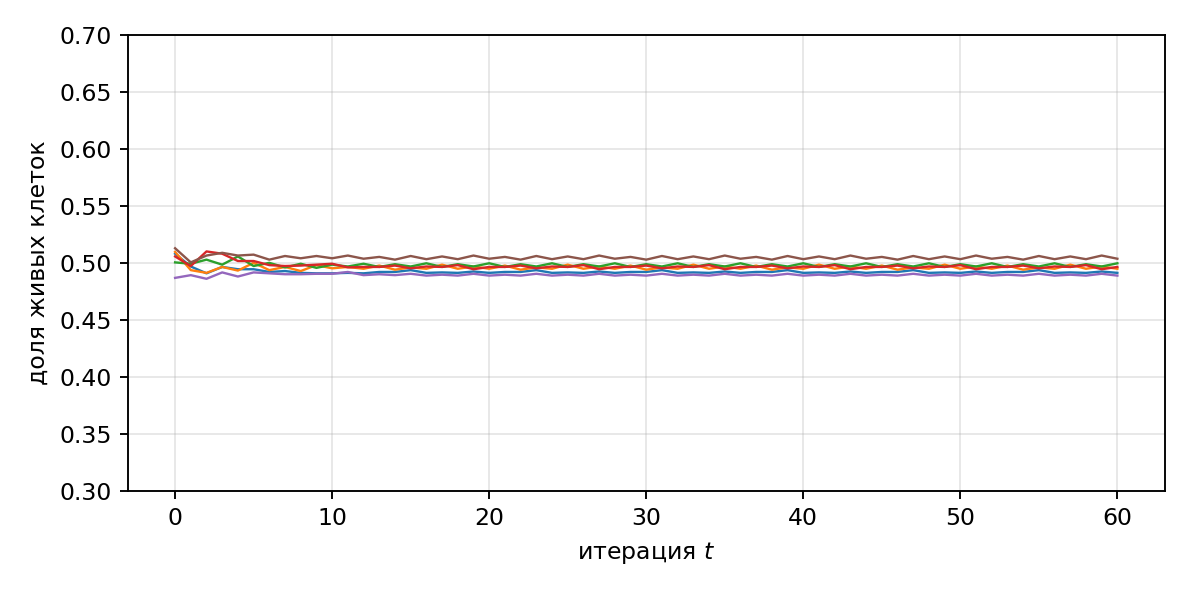
\includegraphics[width=0.75\textwidth]{pic/density.png}
%  \caption{Доля живых клеток при шести случайных стартах, поле $50\times 50$}
%  \label{fig:density}
% \end{figure}

% \begin{figure}[H]
%  \centering
%  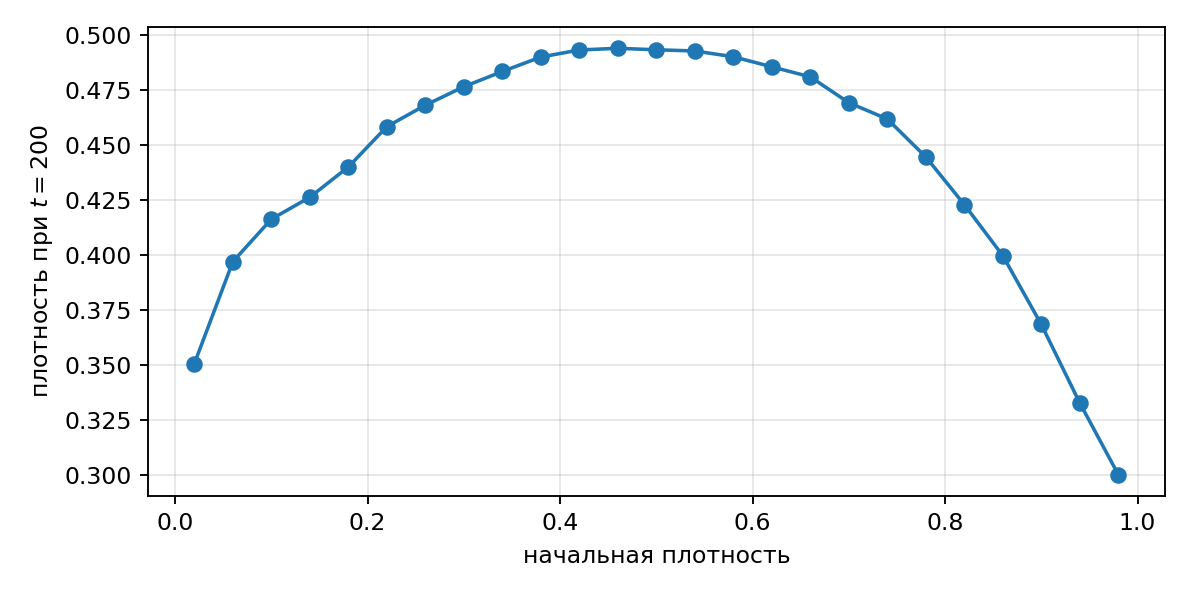
\includegraphics[width=0.75\textwidth]{pic/density_vs_init.png}
%  \caption{Плотность при $t=200$ в зависимости от начальной плотности (поле $40\times 40$, среднее по 15 запускам)}
%  \label{fig:density_init}
% \end{figure}

% Наблюдения:
% \begin{enumerate}[itemsep=-3pt]
%  \item Автомат всегда сходится не к неподвижной точке, а к \textbf{циклу}; ни одна случайная конфигурация не привела к вырождению в пустое или заполненное поле.
%  \item Предпериод короток и растет очень медленно (порядка $10$-$13$ шагов при росте $n$ с $20$ до $50$), т.е. локальный порядок формируется быстро, независимо от размеров поля.
%  \item \textbf{Период в 100\,\% наблюдавшихся запусков кратен ширине поля $n$} (например, $20$, $40$ для $n=20$; $60$, $120$ для $n=30$; $100$, $200$ для $n=50$). Это означает, что устойчивые структуры не стоят на месте, а перемещаются по полю с постоянной скоростью (порядка одной клетки за шаг) и возвращаются в исходное положение, обойдя тор. Тороидальные границы здесь существенны: период определяется длиной «обхода» тора.
% \end{enumerate}

\noindent{\Large \textbf{\subsection{Классификация по Вольфраму}}} \par

По наблюдаемому поведению автомат следует отнести к классу II, так как из случайного начального состояния он за короткое время переходит к набору периодических структур. Однако данная классификация носит оценочный характер, так как строгих критериев классификации Вольфрама не существует.

\newpage
